\documentclass[aspectratio=169]{beamer} %format: 16:9


% Alternatively, select ngerman
\usepackage[american]{babel}
%\usepackage[ngerman]{babel}

% For beginners: themes need to be in the same directory as this tex-file. For experts: no explanation required. ;)
\usetheme{ITD1}
% Choose whether you want the logo on each frame title. Can be changed at any
% time. Note: It adds some vertical white space to the frame's content pane.
\withoutframelogo
%\withoutframelogo

\usepackage{csquotes}
\usepackage{derivative}
\usepackage[
  backend=biber,
  doi=true,
  eprint=false,
  date=iso,
  seconds=true,
  style=alphabetic-verb,
  locallabelwidth=true,
  maxnames = 99,
  %citestyle=alphabetic-verb
  ]{biblatex}
\renewcommand*{\bibfont}{\footnotesize}

\addbibresource{literature.bib}
%\addbibresource{jrcisia-related.bib}

%\addglobalbib{strings-short.bib}
%\addbibresource[label=jrcisia-published]{jrcisia-published.bib}



\title{An Experimental Analysis of the Influence of the Precision of Parameters in an Artificial Neural Network}
% Uncomment if unwanted
\subtitle{Natural Computation PS Presentation 01}

% \author[J. Doe, J. Doe]{Jane Doe, John Doe}
\author[D. K., E. R., S. A. S., L. S.]{Denise Katritschenko, Elias Reich, Sayed Abozar Sadat, Lukas Schwaiger}
% \institute[\isiashort, \fhshort]{\isialong\\ \depitlong\\ \fhlong}
% \institute[\fhshort]{\isialong\\ \depitlong\\ \fhlong}
\institute[\plusshort]{\pluslong\\ Department of Artificial Intelligence and Human Interfaces (AIHI)}
\date[\today]{\today}


% Automatically add fullframe for section headers. Uncomment if you do not want
% them.
\AtBeginSection[]{\fullframe{\insertsectionhead}}

\begin{document}

\frame{\titlepage}
\begin{frame}{Distribution of weight values}
  \begin{itemize}
    \item What values do weights take?
    \item Does ''quantization'' of the fractional part impact model performance?
  \end{itemize}

  \begin{figure}
    \centering  
    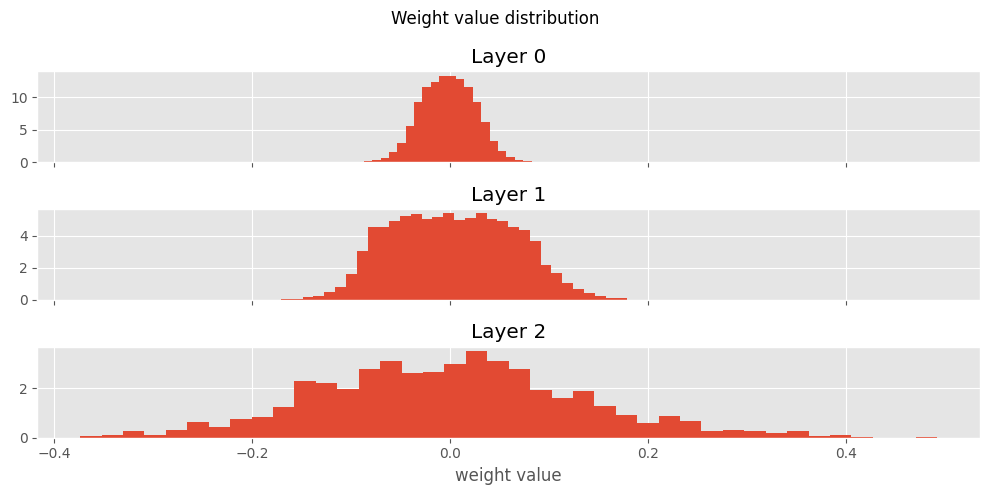
\includegraphics[width=0.8\textwidth]{figures/118_dist.png}
  \end{figure}
\end{frame}

\begin{frame}{Distribution of weight values}
  \begin{itemize}
    \item What values do weights take?
    \item Does ''quantization'' of the fractional part impact model performance?
  \end{itemize}

  \begin{figure}
    \centering  
    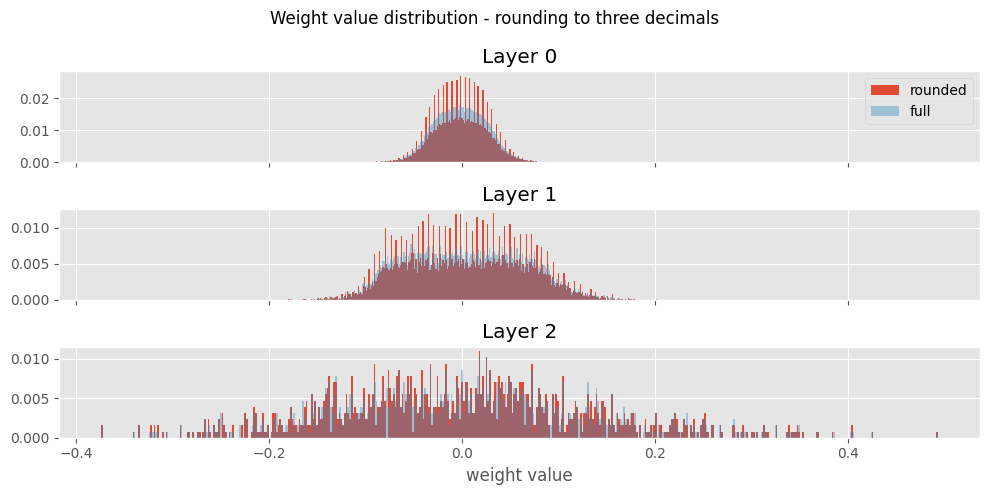
\includegraphics[width=0.8\textwidth]{figures/118_dist3.png}
  \end{figure}
\end{frame}

\begin{frame}{Distribution of weight values}
  \begin{itemize}
    \item What values do weights take?
    \item Does ''quantization'' of the fractional part impact model performance?
  \end{itemize}

  \begin{figure}
    \centering  
    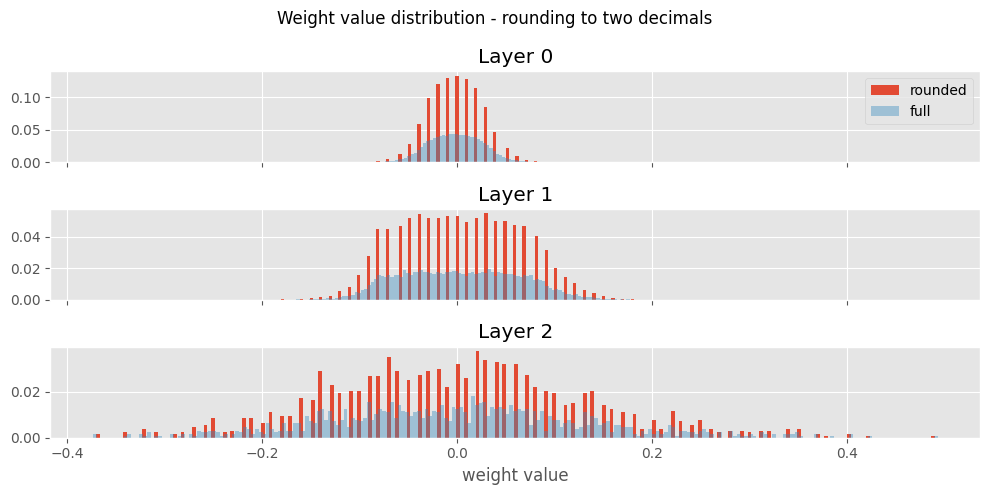
\includegraphics[width=0.8\textwidth]{figures/118_dist2.png}
  \end{figure}
\end{frame}

\begin{frame}{Distribution of weight values}
  \begin{itemize}
    \item What values do weights take?
    \item Does ''quantization'' of the fractional part impact model performance?
  \end{itemize}

  \begin{figure}
    \centering  
    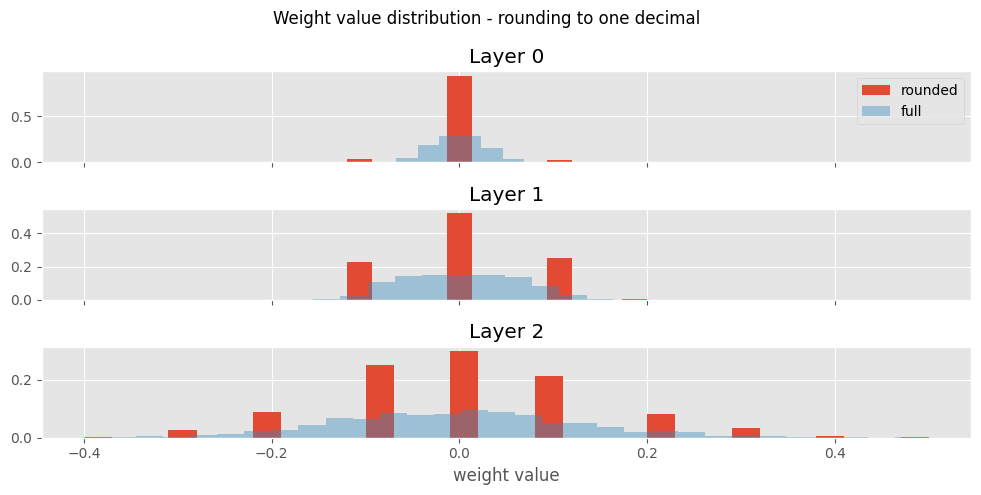
\includegraphics[width=0.8\textwidth]{figures/118_dist1.png}
  \end{figure}
\end{frame}

\begin{frame}{Results}
  \begin{enumerate}
    \item Train a model with fp32.
    \item Round to $n$ decimals.
    \item Profit.
  \end{enumerate}

  \begin{figure}
    \centering  
    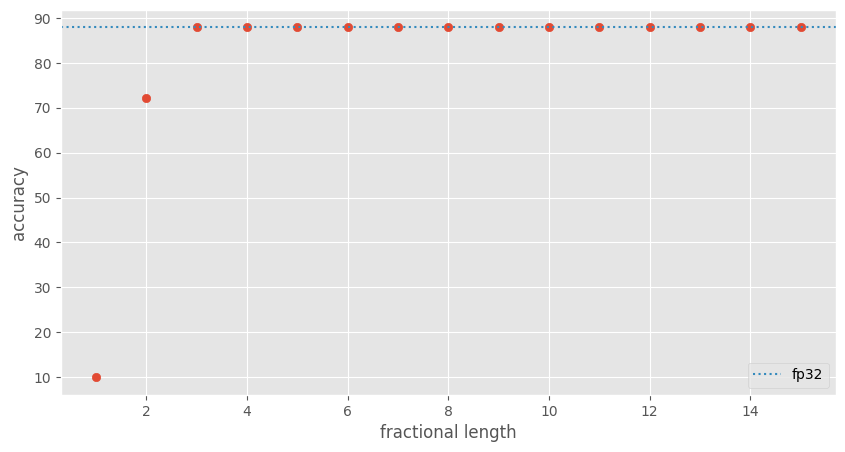
\includegraphics[width=0.75\textwidth]{figures/118_accuracy.png}
  \end{figure}
\end{frame}

\begin{frame}{Results}
  \begin{itemize}
    \item With just 3 decimals we can achieve full fp32 results.
    \item Keep in mind that the data is still fp32.
    \item All operations are still fp32.

    \pause
    \bigskip
    
    \item But! With just 3 decimals, for numbers $\in (-1, 1)$, we only need to store 3 digits.
    \item This can be done with just $10~~(+1)$ bits!
  \end{itemize}
\end{frame}

\fullframe{Thank you}

\end{document}
